% =============================
% FIGURE: Selection map across priorities (no macros, fully explicit)
% Needs: \usepackage{pgfplots} \pgfplotsset{compat=1.18}
% =============================
\begin{figure}[htbp]
\centering
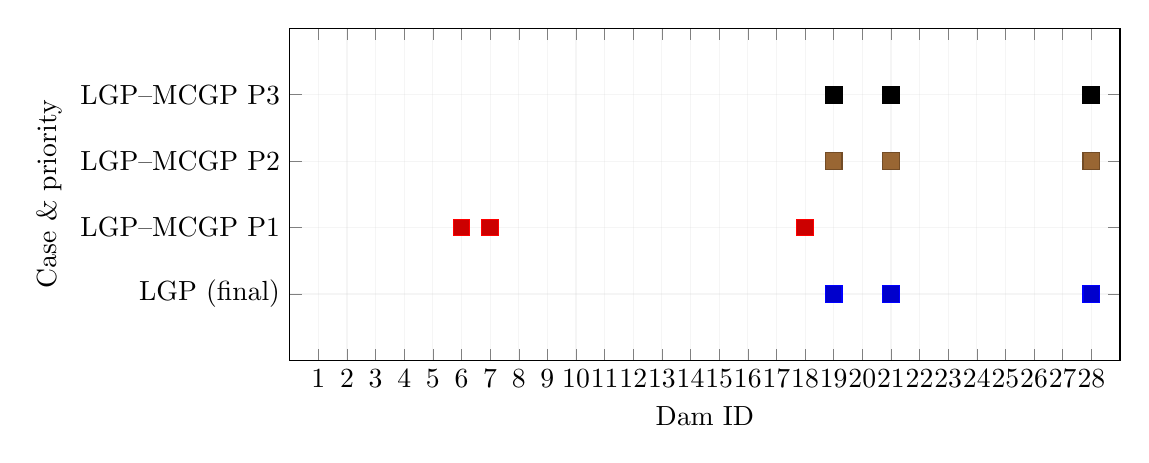
\begin{tikzpicture}
\begin{axis}[
  width=\textwidth, height=5.8cm,
  xmin=0, xmax=29, ymin=0, ymax=5, % integers -> robust parsing
  xlabel={Dam ID}, ylabel={Case \& priority},
  ytick={1,2,3,4},
  yticklabels={LGP (final), LGP--MCGP P1, LGP--MCGP P2, LGP--MCGP P3},
  xtick={1,2,...,28},
  grid=both, grid style={opacity=0.15},
  enlargelimits=false,
]

% Row 1: LGP (final) -> {19,21,28}
\addplot+[only marks,mark=square*,mark size=3pt]
  coordinates {(19,1) (21,1) (28,1)};

% Row 2: LGP–MCGP P1 -> {6,7,18}
\addplot+[only marks,mark=square*,mark size=3pt]
  coordinates {(6,2) (7,2) (18,2)};

% Row 3: LGP–MCGP P2 -> {19,21,28}
\addplot+[only marks,mark=square*,mark size=3pt]
  coordinates {(19,3) (21,3) (28,3)};

% Row 4: LGP–MCGP P3 -> {19,21,28}
\addplot+[only marks,mark=square*,mark size=3pt]
  coordinates {(19,4) (21,4) (28,4)};

\end{axis}
\end{tikzpicture}
\caption{Selected-dam map across LGP baseline and LGP–MCGP priorities. Filled squares mark dams included in each portfolio.}
\label{fig:lgpmc_selection_map}
\end{figure}
